\documentclass[conference]{IEEEtran}
\usepackage{enumitem}
\usepackage{siunitx}
\usepackage{multicol}
\usepackage{array}
\usepackage{multirow}
\usepackage{adjustbox}
\usepackage[table]{xcolor}
\usepackage{colortbl}

\usepackage{caption}
\usepackage{amsfonts}
\usepackage{algorithm,algpseudocode}
\usepackage{lipsum}
\usepackage[flushleft]{threeparttable}

\usepackage{cite}
\usepackage{graphicx}
\graphicspath{{../../assets/}}
\usepackage{amsmath}
\usepackage{array}
\ifCLASSOPTIONcompsoc
 \usepackage[caption=false,font=normalsize,labelfont=sf,textfont=sf]{subfig}
\else
 \usepackage[caption=false,font=footnotesize]{subfig}
\fi
\usepackage{float}
\usepackage{url}

% \hyphenation{op-tical net-works semi-conduc-tor}

\usepackage{algorithm,algpseudocode}
\usepackage{lipsum}

\makeatletter
\newenvironment{breakablealgorithm}
  {% \begin{breakablealgorithm}
   \begin{center}
     \refstepcounter{algorithm}% New algorithm
     \hrule height.8pt depth0pt \kern2pt% \@fs@pre for \@fs@ruled
     \renewcommand{\caption}[2][\relax]{% Make a new \caption
       {\raggedright\textbf{\fname@algorithm~\thealgorithm} ##2\par}%
       \ifx\relax##1\relax % #1 is \relax
         \addcontentsline{loa}{algorithm}{\protect\numberline{\thealgorithm}##2}%
       \else % #1 is not \relax
         \addcontentsline{loa}{algorithm}{\protect\numberline{\thealgorithm}##1}%
       \fi
       \kern2pt\hrule\kern2pt
     }
  }{% \end{breakablealgorithm}
     \kern2pt\hrule\relax% \@fs@post for \@fs@ruled
   \end{center}
  }
\makeatother

\begin{document}
\title{Fast Parallel Image Rotation Algorithm}
\author {
    Dhrubajyoti Mandal \\
    \textit{School of Computer Engineering} \\
    \textit{Kalinga Institute of Industrial Technology} \\
    Bhubaneswar, India \\
    22053859@kiit.ac.in \\ \\ \\
    Sourav Kumar Parida \\
    \textit{School of Computer Engineering} \\
    \textit{Kalinga Institute of Industrial Technology} \\
    Bhubaneswar, India \\
    22051032@kiit.ac.in \\ \\
    Subhadeep Bhadra \\
    \textit{School of Computer Engineering} \\
    \textit{Kalinga Institute of Industrial Technology} \\
    Bhubaneswar, India \\
    2205336@kiit.ac.in
    \and
    Dr. Sujoy Dutta \\
    \textit{Asst. Prof. \& Asst. CoE} \\
    \textit{School of Computer Engineering} \\
    \textit{Kalinga Institute of Industrial Technology} \\
    Bhubaneswar, India \\
    sdattafcs@kiit.ac.in \\ \\
    Chiranjeev Bhaya \\
    \textit{Lead Engineer (Camera System)} \\
    \textit{Samsung R\&D Institute} \\
    Bangalore, India \\
    c.bhaya@samsung.com \\ \\
    Chandra Mohan V \\
    \textit{Architect (Camera System)} \\
    \textit{Samsung R\&D Institute} \\
    Bangalore, India \\
    chandra.mv@samsung.com
}
\maketitle
\begin{abstract}
    This paper presents a novel fast image rotation algorithm that leverages CPU parallelization while maintaining high image quality. The proposed method is a single-pass algorithm, derived from the existing Double-Line Rotation (DLR) method, which reduces computational complexity and generalizes the algorithm. Initially, a baseline for the given image is calculated to determine the starting line, which defines the initial point for each vertical or horizontal line in the image to be rotated. The corresponding pixels to be mapped are identified using floating point arithmetic, and trigonometric calculations are performed only once per line. This approach ensures precise image transformation with minimal computational overhead.
    \textit{Index terms:} Image rotation, line rotation image transform, double-line rotation (DLR), parallel image rotation.
\end{abstract}
\IEEEpeerreviewmaketitle
\section{Introduction}
2-D Image Rotation has a number of applications in digital photography and image processing like image matching, alignment, \cite{gaster2012heterogeneous} etc. Highly accurate image rotation is essential for certain image processing tasks such as feature extraction and matching. Whilst there are many state-of-the-art image rotation algorithms, they have limitations in terms of image quality and speed \cite{ashtari2015double} \cite{park2009accurate}.
Parallel algorithms for image processing aim to execute faster than sequential algorithms, however designing and scheduling a fast parallel image rotation is a challenge \cite{kwon2016study}.
The most straightforward, and perhaps the most well known approach to implement image rotation is by using the rotation matrix \cite{evans2001rotations}, as described here
$$\begin{bmatrix}
        x' \\
        y'
    \end{bmatrix} = \begin{bmatrix}
        x - cx \\
        y - cy
    \end{bmatrix} * \begin{bmatrix}
        cos(\theta) & -sin(\theta) \\
        sin(\theta) & cos(\theta)
    \end{bmatrix}$$\\
where, $\theta$ is the angle of rotation, $x'$ and $y'$ are the new coordinates of the rotated image, and $(cx, cy)$ is the center of the original image, which is treated as the axis of rotation.\\
Assuming the centre of rotation of the new image is $(cx', cy')$, the final new coordinates are:
$$\begin{bmatrix}
        x' \\
        y'
    \end{bmatrix} = \begin{bmatrix}
        x' + cx' \\
        y' + cy'
    \end{bmatrix}$$

% %%%%%%%%%%%%%%%%%%%%%%%%%%%%%%%%%%%%%%%%%%%%%%%%%%%%%%%%%%%%%%%%%%%%


\section{Literature Review}

Affine transformation is a fundamental technique in computer graphics and computational geometry, extensively employed for various image manipulation operations such as translation, scaling, rotation, shearing, and reflection. Mathematically, it is represented as
$ y = Ax + b $ where $A$ is a $2 \times 2$ matrix that defines the linear transformation, and $b$ is a translation vector. This formulation ensures the preservation of geometric properties such as points, straight lines, and planes, making affine transformation indispensable for numerous graphical applications. In the context of image rotation, the matrix $\mathbf{A}$ is typically determined using trigonometric functions based on the rotation angle $\theta$, while the translation components $t_x$ and $t_y$ are calculated to center the rotated image within its new dimensions. The \texttt{warpAffine} function in OpenCV is widely utilized to perform such affine transformations efficiently, offering flexibility in handling various interpolation methods like nearest-neighbor, bilinear, and bicubic. These interpolation methods are crucial for minimizing distortions and preserving image quality during the transformation \cite{wang2021panoramic}.

However, affine transformations are not without limitations, especially when dealing with large rotation angles or combined transformations, such as scaling and shearing, which can lead to artifacts like aliasing and loss of detail. 


To mitigate these issues, more sophisticated methods have been developed. One such method is the Hermite polynomial expansion, which leverages the orthogonality of Hermite polynomials to achieve smooth and accurate interpolation. This technique is particularly effective for image processing tasks requiring high precision. The image function is expanded using two-dimensional Hermite polynomials, and rotation is performed by transforming the coordinates with a rotation matrix. The rotated image is then reconstructed using inverse Hermite expansion, ensuring smooth transitions and minimal distortion. Despite its accuracy, the Hermite expansion method is computationally intensive, requiring the evaluation and summation of multiple polynomial terms, which can result in slower processing times. Additionally, while this method excels at smooth interpolation, it may struggle to maintain fine details in images with high-frequency content \cite{park2009accurate}.

Another advanced technique is the Double Line Rotation (DLR) method, which is recognized for its ability to maintain geometric and intensity integrity during transformation. The DLR method divides the image into eight distinct zones, each governed by specific rotation equations and transformations. This zonal approach ensures that each pixel in the original image is mapped to two corresponding pixels in the rotated image, maintaining a consistent distance ratio between points. This feature is crucial for applications that require feature extraction invariance, making the DLR method particularly suitable for pattern recognition and computer vision tasks. However, the complexity of managing multiple zones and their corresponding transformations can lead to inefficiencies, especially with high-resolution images. Moreover, distortions may occur at the boundaries between zones, potentially degrading the visual quality of the rotated image \cite{ashtari2015double}.

%%%%%%%%%%%%%%%%%%%%%%%%%%%%%%%%%%%%%%%%%%%%%%%%%%%%%%%%%%%%%%%%%%%%%%%%%%%%%%%%%%%%%%%%%%%%%%%%%%%%%%%%%%%


\section{Proposed Method}
The proposed method is a single pass algorithm, which means that it performs the entire image rotation operation at once. The proposed algorithm predominantly affects pixels in the row major (width), or ones in the column major (height), depending on the angle of rotation, $\alpha$.
If $\alpha \in \left ( \frac{\pi}{4}, \frac{3 \pi}{4} \right ] \bigcup \left ( \frac{5 \pi}{4}, \frac{7 \pi}{4} \right ]$, rotation is performed in the \textit{\textbf{column major}}, and it is performed in the \textit{\textbf{row major}} for the rest of the angles. Accordingly, for rotating the source image, entire row or column vectors of pixels are rotated as a single unit, instead of the more common approach, where each individual pixel is separately mapped. Due to this reason, it is necessary to accurately determine the initial coordinates from which the new row or column vector will begin. The coordinates of the rest of the pixels in the vector can then be determined by simple floating point addition or subtraction, depending on the extent to which each of the said vectors are spread across the coordinate axes.

Apart from this, depending on $\alpha$, the pixel processing order changes - i.e., whether the last row or column vector of pixels get processed first, or last. Since it has been found out that these values are very sensitive to $\alpha$, the specific details of which are discussed in the later parts of this paper.
\subsection{Rotation Of An Image In The Column Major} \label{col_major_rotation}





% FIGURE

\begin{figure}[H]
    \centering
    \captionsetup{justification=centering,margin=0.7cm}
    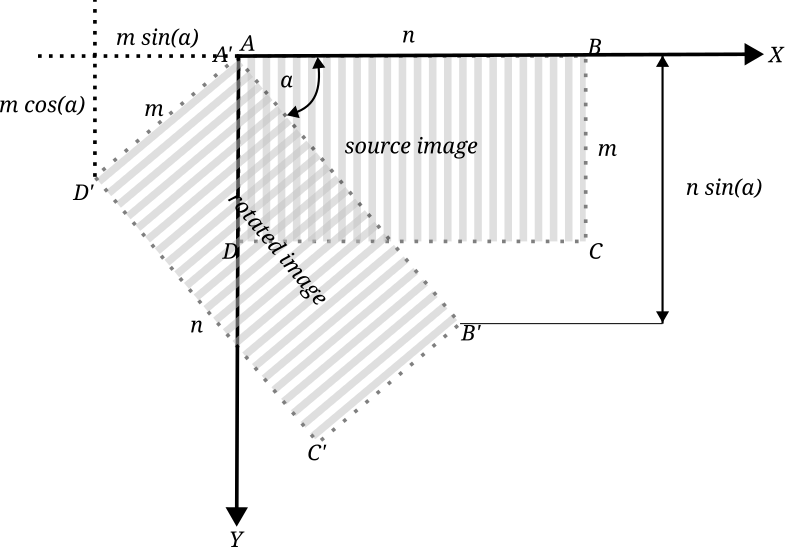
\includegraphics[width=0.5\textwidth]{rotation_example_1.png}
    \caption{Example demonstrating rotation of an image in the column major. Every column vector of pixels are rotated at once (Represented by the stripes in the image).}
    \label{fig:rotation_example_1}
\end{figure}










As seen in the example image in figure \ref{fig:rotation_example_1}, for the given angle of rotation, column vectors were rotated (represented by the stripes). Each such vector to be rotated begins from the line $\overrightarrow{A'B'}$. As such, the initial coordinates of each of these vectors can be determined by the equation of the same line, which is given by:
\begin{equation}
    \label{start_line_eq}
    f(i) = \left\lfloor \frac{i}{tan(\alpha)} \right\rfloor \forall \{i \in \mathbb{Z},\> i \in \left[ 0, n \cdot sin(\alpha) \right)\}
\end{equation}
Thus, the initial coordinates of the column vectors would be of the type $(f(i), i)$. Next, to determine the coordinates of the rest of the pixels in the column vector, as mentioned previously, we perform floating point addition or subtraction, depending on the extent to which each of the said vectors are spread across the coordinate axes.\\
In the example in figure \ref{fig:rotation_example_1}, we can see that each column vector is spread through a length of $m \cdot \sin(\alpha)$ in the $x$-axis and through a length of $m \cdot \cos(\alpha)$ in the $y$-axis. It may also be observed that these values are the projections of any line perpendicular to line defined by the function in equation \ref{start_line_eq} on the coordinate axes.\\
We now define:
$$\delta x = \left\lvert sin(\alpha)\right\rvert$$
$$\delta y = \left\lvert cos(\alpha)\right\rvert$$
The coordinates of the next pixel in the column vector is then given by:
$$(f(i) + \delta x, i + \delta y)$$
The coordinates of the pixel following that is determined by adding $\delta x$ and $\delta y$ to the previous coordinates accordingly, and so on, for each of the $m$ pixels in the given column vector. The end-result is that this operation covers all the $m \cdot \sin(\alpha)$ pixels in the $x$-axis and all the $m \cdot \cos(\alpha)$ pixels in the $y$-axis, therefore mapping all of the $m$ pixels in the specific column vector.\\
This process continues for all of the $n$ column vectors in the image, until the entire image is rotated. In practice, each column vector is actually mapped \textbf{twice}. The first mapping happens from the $i\>th$ column vector in $I$ to the $i\>th$ column vector in $R$. The second mapping happens from the $i\>th$ column vector in $I$ to the $(i+1)\>th$ column vector in $R$. Each of these $(i+1)\>th$ column vectors get overwitten in each iteration with a new column vector in $I$; however, this gives a sufficiently accurate issusion of anti-aliasing without losing much quality.

The signs for $\delta x$ and $\delta y$ depend on whether, while mapping the column vectors in the rotated image, the values of the $x$-coordinate $y$-coordinate are decreasing or increasing. In the given example in figure \ref{fig:rotation_example_1}, $\delta x$ is negative, but $\delta y$ is positive.\\
There is a third parameter, defined as:
$$\delta i = \frac{1}{\delta x}$$
$\delta i$ determines the rate at which the column vector is processed from one to the next, and its sign depends on the angle of rotation, $\alpha$.
The calculations for $\delta x$, $\delta y$, and $\delta i$ only happen once per column vector in the image, so the entire image transformation is quite fast, overall.
\subsection{Rotation Of An Image In The Row Major} \label{row_major_rotation}
\begin{figure}[H]
    \centering
    \captionsetup{justification=centering,margin=0.7cm}
    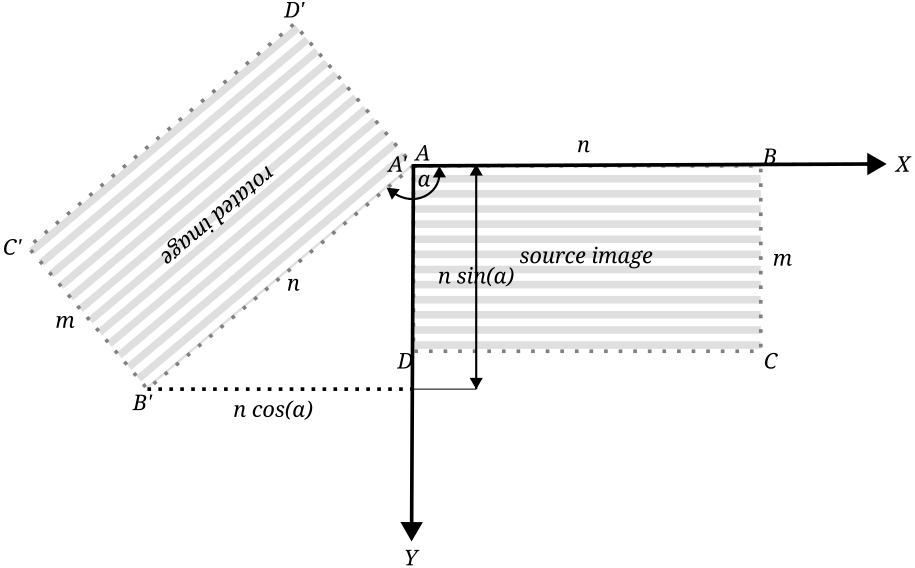
\includegraphics[width=0.5\textwidth]{rotation_example_2.png}
    \caption{Example demonstrating rotation of an image in the row major. Every row vector of pixels are rotated at once (Represented by the stripes in the image).}
    \label{fig:rotation_example_2}
\end{figure}
In the example image in figure \ref{fig:rotation_example_2}, for the given angle of rotation, row vectors were rotated (represented by the stripes). All the calculations and logic is very similar to the one described for rotation in the column major [\ref{col_major_rotation}]. Here, each vector to be rotated begins from the line $\overrightarrow{A'D'}$, whose equation is given by:
\begin{equation}
    \label{start_line_eq_2}
    f(i) = \left\lfloor \frac{i}{tan(\alpha + \frac{\pi}{2})} \right\rfloor \forall \{i \in \mathbb{Z},\> i \in \left[ 0, m \cdot cos(\alpha) \right)\}
\end{equation}
Everything else stays the same, except the fact that now, each row vector is spread through a length of $n \cdot \cos(\alpha)$ in the $x$-axis and through a length of $n \cdot \sin(\alpha)$ in the $y$-axis, and accordingly, we have:
$$\delta x = \left\lvert cos(\alpha)\right\rvert$$
$$\delta y = \left\lvert sin(\alpha)\right\rvert$$


\begin{table}[t]
    \begin{threeparttable}
        \caption{Notation}
        \label{table:notations}
        \centering
        \begin{tabular}{|m{1.5cm}|m{6cm}|}
            \hline
            \textbf{Symbol}  & \textbf{Description}                                                                                                                        \\
            \hline
            $I$              & Original image                                                                                                                              \\ \hline
            $m, n$           & Height, width of $I$                                                                                                                        \\ \hline
            $R$              & Rotated image                                                                                                                               \\ \hline
            $m', n'$         & Height, width of $R$                                                                                                                        \\ \hline
            $\alpha$         & Angle of rotation in radians                                                                                                                \\ \hline
            $x'$             & Offset by which the $x$-coordinates of $R$ need to be shifted                                                                               \\ \hline
            $y'$             & Offset by which the $y$-coordinates of $R$ need to be shifted                                                                               \\ \hline
            $f(...)$         & Function defining the equation of the line from where the row or column vector starts [eq. \ref{start_line_eq}] [eq. \ref{start_line_eq_2}] \\ \hline
            $r_o$            & Upper limit of the function $f$                                                                                                             \\ \hline
            $N$              & Number of elements (pixels) in the row or column vector $f$                                                                                 \\ \hline
            \verb|flip|      & Boolean value that changes pixel processing order based on $\alpha$                                                                         \\ \hline
            \verb|row_major| & Boolean value that determines whether processing is to be done in the row or column major                                                   \\ \hline
            \verb|negate|    & Boolean value, that if true, negates the indices used for indexing the pixels of the image                                                  \\ \hline
        \end{tabular}
        \begin{tablenotes}
            \small
            \item \textbf{Note:} The algorithm described in [Algorithm \ref{rotation_alorithm}] follows \textbf{\textit{Python}} style indexing. For example, if \verb|a = [[1, 2, 3], [5, 6]]|, then \verb|a[0][-1]| represents the element \verb|3|.
        \end{tablenotes}
    \end{threeparttable}
\end{table}


\subsection{Implementation}

\begin{breakablealgorithm} \label{rotation_alorithm}
    \caption{Image Rotation Algorithm}
    \begin{algorithmic}[1]
        \Procedure{rotate}{$...$}\Comment{Performs image rotation on $R$}
        \State \texttt{src\_i} $ = 0$ \Comment{Initialize internal control variables}
        \State \texttt{S} $ = 1$
        \State $M = [\>]$
        \If{\texttt{negate}}
        \State \texttt{S = -1}
        \EndIf

        \If{\texttt{flip}}
        \State $M = [m_i]\> for\> i=0,1,…,N-1,\>|\> m_i=N-i$
        \Else
        \State $M = [m_i]\> for\> i=0,1,…,N-1,\>|\> m_i=N$
        \EndIf

        \For{$i=0$ to $r_o$}
        \State \texttt{temp\_x = } $f(i)$
        \State \texttt{temp\_y = } $i$

        \For{$px$ in $M$}
        \State $x = \lfloor$ \texttt{temp\_x} $\rfloor$
        \State $y = \lfloor$ \texttt{temp\_y} $\rfloor$
        \State \texttt{temp\_i} $= \lfloor$ \texttt{src\_i} $\rfloor$

        \If{\texttt{row\_major}}
        \State $a = $ \texttt{temp\_i}
        \State $b = px$
        \Else
        \State $a = px$
        \State $b = $ \texttt{temp\_i}
        \EndIf

        \Comment{Map rotated pixels to $R$}
        \State $R[$ \texttt{S} $*\> (y + y'),\> $\texttt{ S }$ *\> (x + x')] = I[a, b]$
        \State $R[$ \texttt{S} $*\> (y + y') + 1,\> $\texttt{ S }$ *\> (x + x')] = I[a, b]$

        \State \texttt{temp\_x += } $\delta x$
        \State \texttt{temp\_y += } $\delta y$

        \EndFor

        \State \texttt{src\_i += } $\delta i$
        \EndFor

        \EndProcedure
    \end{algorithmic}
\end{breakablealgorithm}


The algorithm described above [Algorithm \ref{rotation_alorithm}] rotates image $I$ to $R$.\\
$R$ is Initialized as a blank image of width $n'$ and height $m'$ to fit $R$ in the canvas, where:
$$m' = \left\lceil \left\lvert m \cdot cos(\alpha) + n \cdot sin(\alpha) \right\rvert \right\rceil $$
$$n' = \left\lceil \left\lvert m \cdot sin(\alpha) + n \cdot cos(\alpha) \right\rvert \right\rceil $$
The rotation function is then invoked, with each of the parameters updating depending on the value of $\alpha$, as discussed above. The detailed values of each of the parameters are mentioned in [Table \ref{table:rotation_params}].\\ \\
\textbf{Note:} It has been observed, that for ranges of $\alpha$ which are vertically opposite each other (For example, angles in the range $\left ( \frac{\pi}{4}, \frac{\pi}{2} \right ]$ are vertically opposite angles in the range $\left ( \frac{5 \pi}{4}, \frac{ 3 \pi}{2} \right ]$, and so on), the only parameters of rotation that change are $\delta i$, \texttt{negate}, and \texttt{flip}. As such, the calculations have been generalized for such angles and they have been represented in [Table \ref{table:rotation_params}], with a $(')$ at the end of their names (shaded cells).\\


\begin{breakablealgorithm} \label{driver_function}
    \caption{Driver Function}
    \begin{algorithmic}[1]
        \Procedure{main}{$...$}\Comment{Invokes [Algorithm \ref{rotation_alorithm}]}

        \State Determine the boolean value of \texttt{row\_major}
        \State Determine \textit{\textbf{f}}, based on the value of \texttt{row\_major}
        \State Initialize a blank image $R$ with dimensions $(m', n')$

        \State Determine the parameters of rotation from [Table \ref{table:rotation_params}]

        \State Generate $R$ using [Algorithm \ref{rotation_alorithm}]
        \EndProcedure
    \end{algorithmic}
\end{breakablealgorithm}

\renewcommand{\arraystretch}{3}  % This sets the row height to 3 cm
\definecolor{lightgray}{gray}{0.91}
\begin{table*}[h]
    \caption{Rotation Parameters, based on $\alpha$}
    \label{table:rotation_params}
    \centering
    \begin{tabular}{ |p{0.8cm}|p{1.53cm}|p{1.53cm}|p{1.1cm}|p{1.1cm}|p{0.67cm}|p{1.53cm}|p{0.1cm}|p{0.87cm}|p{0.87cm}|>{\columncolor{lightgray}}p{0.67cm}|>{\columncolor{lightgray}}p{0.95cm}|>{\columncolor{lightgray}}p{0.8cm}| }
        \hline
        \raisebox{0ex}{\multirow{2}{*}{\adjustbox{angle=90}{\textbf{Range of $\alpha$}}}} & \multicolumn{12}{c|}{\textbf{Rotation parameters}}                                                                                                                                                                                                                                                                                                                                                                                                    \\
        \cline{2-13}
                                                                                          & \textbf{$x'$}                                                            & \textbf{$y'$}                                                            & \textbf{$\delta x$}                      & \textbf{$\delta y$}                      & \textbf{$\delta i$} & \textbf{$r_o$}                                                           & \textbf{N} & \texttt{negate} & \texttt{flip}  & \textbf{$\delta i'$} & \texttt{negate'} & \texttt{flip'} \\
        \hline
        $\left [ 0, \frac{\pi}{4} \right ]$                                               & $\left\lceil \left\lvert m \cdot \sin(\alpha) \right\rvert \right\rceil$ & 0                                                                        & $\left\lvert \cos(\alpha) \right\rvert$  & $\left\lvert \sin(\alpha) \right\rvert$  & $1 / \delta x$      & $\left\lceil \left\lvert m \cdot \cos(\alpha) \right\rvert \right\rceil$ & n          & \texttt{false}  & \texttt{false} & $1 / \delta x$       & \texttt{true}    & \texttt{false} \\
        \hline
        $\left ( \frac{\pi}{4}, \frac{\pi}{2} \right ]$                                   & $\left\lceil \left\lvert m \cdot \sin(\alpha) \right\rvert \right\rceil$ & 0                                                                        & $-\left\lvert \sin(\alpha) \right\rvert$ & $\left\lvert \cos(\alpha) \right\rvert$  & $-1 / \delta x$     & $\left\lceil \left\lvert n \cdot \sin(\alpha) \right\rvert \right\rceil$ & m          & \texttt{false}  & \texttt{false} & $1 / \delta x$       & \texttt{false}   & \texttt{true}  \\
        \hline
        $\left ( \frac{\pi}{2}, \frac{3 \pi}{4} \right ]$                                 & $m'$                                                                     & $\left\lceil \left\lvert m \cdot \cos(\alpha) \right\rvert \right\rceil$ & $-\left\lvert \sin(\alpha) \right\rvert$ & $-\left\lvert \cos(\alpha) \right\rvert$ & $-1 / \delta x$     & $\left\lceil \left\lvert n \cdot \sin(\alpha) \right\rvert \right\rceil$ & m          & \texttt{false}  & \texttt{false} & $1 / \delta x$       & \texttt{false}   & \texttt{true}  \\
        \hline
        $\left ( \frac{3 \pi}{4}, \pi \right ]$                                           & $\left\lceil \left\lvert n \cdot \cos(\alpha) \right\rvert \right\rceil$ & 0                                                                        & $-\left\lvert \cos(\alpha) \right\rvert$ & $\left\lvert \sin(\alpha) \right\rvert$  & $1 / \delta x$      & $\left\lceil \left\lvert m \cdot \cos(\alpha) \right\rvert \right\rceil$ & n          & \texttt{false}  & \texttt{false} & $1 / \delta x$       & \texttt{true}    & \texttt{false} \\
        \hline
    \end{tabular}
\end{table*}

\newpage

\section{Experimental Results and Analysis}
In this section, we perform an accuracy analysis of the reconstructed images using various error metrics. These metrics quantify the similarity between the original and the processed images, providing insight into the effectiveness of the image processing techniques. The following subsections describe each metric in detail, including their mathematical formulation and interpretation.

% \begin{multicols}{2}

\subsection{Peak Signal-to-Noise Ratio (PSNR)}
PSNR is a widely used metric for evaluating the quality of reconstructed or compressed images. It quantifies the ratio between the maximum possible pixel value of the image and the mean squared error (MSE) between the original and the processed images. PSNR is expressed in decibels (dB), with higher values indicating better image quality.

\begin{equation}
\text{PSNR} = 20 \cdot \log_{10}\left(\frac{\text{MAX}_{I}}{\sqrt{\text{MSE}}}\right)
\end{equation}

The Mean Squared Error (MSE) is calculated as:
\begin{equation}
\text{MSE} = \frac{1}{MN} \sum_{i=1}^{M} \sum_{j=1}^{N} \left[I(i,j) - K(i,j)\right]^2
\end{equation}

where \(\text{MAX}_{I}\) represents the maximum possible pixel value (e.g., 255 for 8-bit images), and \(I(i,j)\) and \(K(i,j)\) are the pixel values at position \((i,j)\) in the original and processed images, respectively.

\subsection{Correlation Coefficient (CC)}
The Correlation Coefficient (CC) is a statistical measure that quantifies the similarity between two images by assessing the correlation between corresponding pixels. CC ranges from -1 to 1, with 1 indicating perfect positive correlation, -1 indicating perfect negative correlation, and 0 indicating no correlation.

\begin{equation}
\text{CC} = \frac{\sum_{i=1}^{M} \sum_{j=1}^{N} \left(I(i,j) - \overline{I}\right) \left(K(i,j) - \overline{K}\right)}{\sqrt{\sum_{i=1}^{M} \sum_{j=1}^{N} \left(I(i,j) - \overline{I}\right)^2 \cdot \sum_{i=1}^{M} \sum_{j=1}^{N} \left(K(i,j) - \overline{K}\right)^2}}
\end{equation}

Here, \(\overline{I}\) and \(\overline{K}\) represent the mean pixel values of the original and processed images, respectively.

\subsection{Laplacian Mean Squared Error (LMSE)}
Laplacian Mean Squared Error (LMSE) focuses on the high-frequency components of an image, particularly edges. By applying a Laplacian filter to both the original and processed images, LMSE calculates the error in edge details, which is particularly useful for detecting blurring or loss of fine details.

\begin{equation}
\text{LMSE} = \frac{1}{MN} \sum_{i=1}^{M} \sum_{j=1}^{N} \left[\text{Laplacian}(I(i,j)) - \text{Laplacian}(K(i,j))\right]^2
\end{equation}

Lower LMSE values indicate less error in edge preservation, thus implying higher image quality.

\subsection{Relative Error (Re)}
Relative Error (Re) quantifies the overall difference between the original and processed images, normalized by the magnitude of the original image's pixel values. This metric is useful for assessing the general accuracy of image reconstruction.

\begin{equation}
\text{Re} = \frac{\sum_{i=1}^{M} \sum_{j=1}^{N} |I(i,j) - K(i,j)|}{\sum_{i=1}^{M} \sum_{j=1}^{N} |I(i,j)|}
\end{equation}

Lower values of Re indicate better similarity between the images.

\subsection{Structural Similarity Index (SSIM)}
The Structural Similarity Index (SSIM) measures the perceptual difference between two images. Unlike MSE-based metrics, SSIM considers changes in structural information, luminance, and contrast, making it more aligned with human visual perception. SSIM ranges from -1 to 1, with 1 indicating identical images.

\begin{equation}
\text{SSIM}(I, K) = \frac{(2\mu_I \mu_K + C_1)(2\sigma_{IK} + C_2)}{(\mu_I^2 + \mu_K^2 + C_1)(\sigma_I^2 + \sigma_K^2 + C_2)}
\end{equation}

In this formula, \(\mu_I\) and \(\mu_K\) are the mean values, \(\sigma_I^2\) and \(\sigma_K^2\) are the variances, and \(\sigma_{IK}\) is the covariance of the original and processed images. The constants \(C_1\) and \(C_2\) are used to stabilize the formula when the denominator is close to zero, typically defined as:

\begin{equation}
C_1 = (k_1 L)^2, \quad C_2 = (k_2 L)^2
\end{equation}

where \(L\) is the dynamic range of the pixel values (e.g., 255 for 8-bit images), and \(k_1\) and \(k_2\) are small constants (e.g., \(k_1 = 0.01\), \(k_2 = 0.03\)).

% \end{multicols}
\begin{table}[htbp]
    \caption{PSNR Error Analysis of Various Sample Images}
    \centering
    \renewcommand{\arraystretch}{1.8} % Adjust row height if needed
    \resizebox{\columnwidth}{!}{ % Resize the table to fit within the column width
        \begin{tabular}{|c|c|c|c|c|c|c|c|}
        \hline
        \multirow{2}{*}{\centering \textbf{Methods}} & \multicolumn{7}{c|}{\textbf{Images}} \\
        \cline{2-8}
        & \textbf{astronaut} & \textbf{brick} & \textbf{chelsea} & \textbf{color} & \textbf{moon} & \textbf{page} & \textbf{text} \\
        \hline
        affine\_transform & 26.33 & 28.50 & 25.72 & 46.74 & 30.84 & 19.00 & 27.66 \\
        \hline
        benchmark\_custom & 24.30 & 26.10 & 24.80 & 43.41 & 30.38 & 17.42 & 25.88 \\
        \hline
        benchmark & 27.83 & 29.83 & 26.33 & 44.62 & 33.84 & 18.61 & 30.73 \\
        \hline
        bicubic & 27.32 & 29.51 & 25.91 & 44.54 & 33.46 & 17.96 & 30.27 \\
        \hline
        lanczos & 27.26 & 29.49 & 25.85 & 44.53 & 33.36 & 17.85 & 30.18 \\
        \hline
        linear & 27.83 & 29.83 & 26.33 & 44.62 & 33.84 & 18.61 & 30.73 \\
        \hline
        nearest & 26.45 & 28.73 & 25.55 & 44.29 & 32.36 & 17.74 & 29.02 \\
        \hline
        proposed\_algorithm & 25.89 & 28.16 & 26.10 & 44.65 & 32.47 & 17.51 & 27.82 \\
        \hline
        \end{tabular}
    }
    \label{tab:error_analysis}
\end{table}






\begin{table}[htbp]
    \caption{NAE Analysis of Various Sample Images}
    \centering
    \renewcommand{\arraystretch}{1.8} % Adjust row height if needed
    \resizebox{\columnwidth}{!}{ % Resize the table to fit within the column width
        \begin{tabular}{|c|c|c|c|c|c|c|c|}
        \hline
        \multirow{2}{*}{\centering \textbf{Methods}} & \multicolumn{7}{c|}{\textbf{Images}} \\
        \cline{2-8}
        & \textbf{astronaut} & \textbf{brick} & \textbf{chelsea} & \textbf{color} & \textbf{moon} & \textbf{page} & \textbf{text} \\
        \hline
        affine\_transform & 0.0518 & 0.0461 & 0.0708 & 0.0134 & 0.0186 & 0.1077 & 0.0455 \\
        \hline
        benchmark\_custom & 0.0789 & 0.0728 & 0.0867 & 0.0212 & 0.0259 & 0.1370 & 0.0680 \\
        \hline
        benchmark & 0.0533 & 0.0489 & 0.0727 & 0.0185 & 0.0179 & 0.1208 & 0.0404 \\
        \hline
        bicubic & 0.0565 & 0.0505 & 0.0772 & 0.0186 & 0.0195 & 0.1312 & 0.0438 \\
        \hline
        lanczos & 0.0573 & 0.0512 & 0.0782 & 0.0186 & 0.0204 & 0.1337 & 0.0453 \\
        \hline
        linear & 0.0533 & 0.0489 & 0.0727 & 0.0185 & 0.0179 & 0.1208 & 0.0404 \\
        \hline
        nearest & 0.0584 & 0.0505 & 0.0776 & 0.0188 & 0.0189 & 0.1312 & 0.0470 \\
        \hline
        proposed\_algorithm & 0.0621 & 0.0548 & 0.0758 & 0.0177 & 0.0194 & 0.1339 & 0.0530 \\
        \hline
        \end{tabular}
    }
    \label{tab:nae_analysis}
\end{table}













\begin{table}[htbp]
    \caption{CC Analysis of Various Sample Images}
    \centering
    \renewcommand{\arraystretch}{1.8} % Adjust row height if needed
    \resizebox{\columnwidth}{!}{ % Resize the table to fit within the column width
        \begin{tabular}{|c|c|c|c|c|c|c|c|}
        \hline
        \multirow{2}{*}{\centering \textbf{Methods}} & \multicolumn{7}{c|}{\textbf{Images}} \\
        \cline{2-8}
        & \textbf{astronaut} & \textbf{brick} & \textbf{chelsea} & \textbf{color} & \textbf{moon} & \textbf{page} & \textbf{text} \\
        \hline
        affine\_transform & 0.9882 & 0.9866 & 0.9786 & 0.9998 & 0.9916 & 0.9542 & 0.9873 \\
        \hline
        benchmark\_custom & 0.9811 & 0.9768 & 0.9735 & 0.9997 & 0.9907 & 0.9339 & 0.9808 \\
        \hline
        benchmark & 0.9916 & 0.9901 & 0.9813 & 0.9997 & 0.9958 & 0.9492 & 0.9937 \\
        \hline
        bicubic & 0.9906 & 0.9894 & 0.9795 & 0.9997 & 0.9954 & 0.9414 & 0.9930 \\
        \hline
        lanczos & 0.9904 & 0.9893 & 0.9792 & 0.9997 & 0.9953 & 0.9399 & 0.9929 \\
        \hline
        linear & 0.9916 & 0.9901 & 0.9813 & 0.9997 & 0.9958 & 0.9492 & 0.9937 \\
        \hline
        nearest & 0.9885 & 0.9873 & 0.9777 & 0.9997 & 0.9941 & 0.9385 & 0.9907 \\
        \hline
        proposed\_algorithm & 0.9869 & 0.9855 & 0.9804 & 0.9997 & 0.9943 & 0.9354 & 0.9877 \\
        \hline
        \end{tabular}
    }
    \label{tab:cc_analysis}
\end{table}






\begin{table}[htbp]
    \caption{MSE Analysis of Various Sample Images}
    \centering
    \renewcommand{\arraystretch}{1.8} % Adjust row height if needed
    \resizebox{\columnwidth}{!}{ % Resize the table to fit within the column width
        \begin{tabular}{|c|c|c|c|c|c|c|c|}
        \hline
        \multirow{2}{*}{\centering \textbf{Methods}} & \multicolumn{7}{c|}{\textbf{Images}} \\
        \cline{2-8}
        & \textbf{astronaut} & \textbf{brick} & \textbf{chelsea} & \textbf{color} & \textbf{moon} & \textbf{page} & \textbf{text} \\
        \hline
        affine\_transform & 151.39 & 91.94 & 174.41 & 1.38 & 53.63 & 818.37 & 111.37 \\
        \hline
        benchmark\_custom & 241.41 & 159.73 & 215.49 & 2.97 & 59.56 & 1177.32 & 168.09 \\
        \hline
        benchmark & 107.27 & 67.63 & 151.36 & 2.24 & 26.86 & 895.08 & 55.02 \\
        \hline
        bicubic & 120.48 & 72.81 & 166.61 & 2.28 & 29.31 & 1041.21 & 61.04 \\
        \hline
        lanczos & 122.28 & 73.18 & 169.12 & 2.29 & 30.01 & 1067.74 & 62.34 \\
        \hline
        linear & 107.27 & 67.63 & 151.36 & 2.24 & 26.86 & 895.08 & 55.02 \\
        \hline
        nearest & 147.27 & 87.07 & 180.97 & 2.42 & 37.75 & 1095.27 & 81.52 \\
        \hline
        proposed\_algorithm & 167.41 & 99.41 & 159.55 & 2.23 & 36.80 & 1153.37 & 107.45 \\
        \hline
        \end{tabular}
    }
    \label{tab:mse_analysis}
\end{table}






\begin{table}[htbp]
    \caption{RE Analysis of Various Sample Images}
    \centering
    \renewcommand{\arraystretch}{1.8} % Adjust row height if needed
    \resizebox{\columnwidth}{!}{ % Resize the table to fit within the column width
        \begin{tabular}{|c|c|c|c|c|c|c|c|}
        \hline
        \multirow{2}{*}{\centering \textbf{Methods}} & \multicolumn{7}{c|}{\textbf{Images}} \\
        \cline{2-8}
        & \textbf{astronaut} & \textbf{brick} & \textbf{chelsea} & \textbf{color} & \textbf{moon} & \textbf{page} & \textbf{text} \\
        \hline
        affine\_transform & 0.0518 & 0.0461 & 0.0708 & 0.0134 & 0.0186 & 0.1077 & 0.0455 \\
        \hline
        benchmark\_custom & 0.0789 & 0.0728 & 0.0867 & 0.0212 & 0.0259 & 0.1370 & 0.0680 \\
        \hline
        benchmark & 0.0533 & 0.0489 & 0.0727 & 0.0185 & 0.0179 & 0.1208 & 0.0404 \\
        \hline
        bicubic & 0.0565 & 0.0505 & 0.0772 & 0.0186 & 0.0195 & 0.1312 & 0.0438 \\
        \hline
        lanczos & 0.0573 & 0.0512 & 0.0782 & 0.0186 & 0.0204 & 0.1337 & 0.0453 \\
        \hline
        linear & 0.0533 & 0.0489 & 0.0727 & 0.0185 & 0.0179 & 0.1208 & 0.0404 \\
        \hline
        nearest & 0.0584 & 0.0505 & 0.0776 & 0.0188 & 0.0189 & 0.1312 & 0.0470 \\
        \hline
        proposed\_algorithm & 0.0621 & 0.0548 & 0.0758 & 0.0177 & 0.0194 & 0.1339 & 0.0530 \\
        \hline
        \end{tabular}
    }
    \label{tab:re_analysis}
\end{table}



\begin{table}[htbp]
    \caption{SSIM Analysis of Various Sample Images}
    \centering
    \renewcommand{\arraystretch}{1.8} % Adjust row height if needed
    \resizebox{\columnwidth}{!}{ % Resize the table to fit within the column width
        \begin{tabular}{|c|c|c|c|c|c|c|c|}
        \hline
        \multirow{2}{*}{\centering \textbf{Methods}} & \multicolumn{7}{c|}{\textbf{Images}} \\
        \cline{2-8}
        & \textbf{astronaut} & \textbf{brick} & \textbf{chelsea} & \textbf{color} & \textbf{moon} & \textbf{page} & \textbf{text} \\
        \hline
        affine\_transform & 0.9352 & 0.9354 & 0.8363 & 0.9929 & 0.9555 & 0.7894 & 0.9136 \\
        \hline
        benchmark\_custom & 0.8812 & 0.8794 & 0.7790 & 0.9893 & 0.9276 & 0.6919 & 0.8428 \\
        \hline
        benchmark & 0.9390 & 0.9402 & 0.8222 & 0.9921 & 0.9619 & 0.7269 & 0.9273 \\
        \hline
        bicubic & 0.9335 & 0.9367 & 0.8088 & 0.9917 & 0.9574 & 0.7095 & 0.9174 \\
        \hline
        lanczos & 0.9317 & 0.9354 & 0.8059 & 0.9916 & 0.9557 & 0.7030 & 0.9134 \\
        \hline
        linear & 0.9390 & 0.9402 & 0.8222 & 0.9921 & 0.9619 & 0.7269 & 0.9273 \\
        \hline
        nearest & 0.9218 & 0.9281 & 0.8040 & 0.9904 & 0.9507 & 0.7079 & 0.9014 \\
        \hline
        proposed\_algorithm & 0.9148 & 0.9185 & 0.8095 & 0.9902 & 0.9483 & 0.7090 & 0.8837 \\
        \hline
        \end{tabular}
    }
    \label{tab:ssim_analysis}
\end{table}


\section{Conclusion}
The conclusion goes here.
\section*{Acknowledgment}
The authors would like to thank...

\bibliography{references}
\bibliographystyle{ieeetr}


\end{document}
